\documentclass{standalone}

\usepackage{tikz, pgfplots} % for 2D and 3D graphics
\pgfplotsset{compat=1.15}

\definecolor{ocre}{RGB}{0,83,166}

\begin{document}

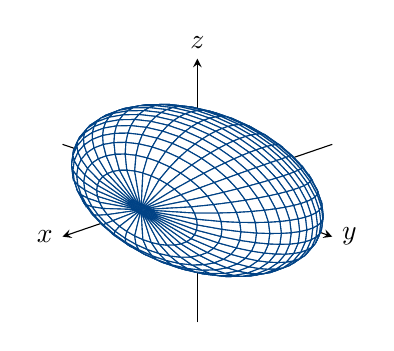
\begin{tikzpicture}
\begin{axis}
[view={135}{20},colormap={ocre}{
            color=(ocre) color=(ocre)
        },
axis lines=center,axis on top,
ticks=none,set layers=default,axis equal,
xlabel={$x$}, ylabel={$y$}, zlabel={$z$},
xlabel style={anchor=east},
ylabel style={anchor=west},
zlabel style={anchor=south},
enlargelimits,
tick align=inside,
domain=0:2.00,
samples=20, 
z buffer=sort,
]
\addplot3 [surf,draw=ocre!30,fill=white,samples=20, domain=-1:1, domain y=0:180, on layer=axis foreground] ({x}, {-2*cos(y)*sqrt(1-x^2)}, {-sin(y)*sqrt(1-x^2)});
\addplot3 [surf,draw=ocre!30,fill=white,domain=-1:1,samples=20, domain y=0:180,on layer=axis foreground] ({x},{2*cos(y)*sqrt(1-x^2)},{sin(y)*sqrt(1-x^2)});
\end{axis}
\end{tikzpicture}

\end{document}